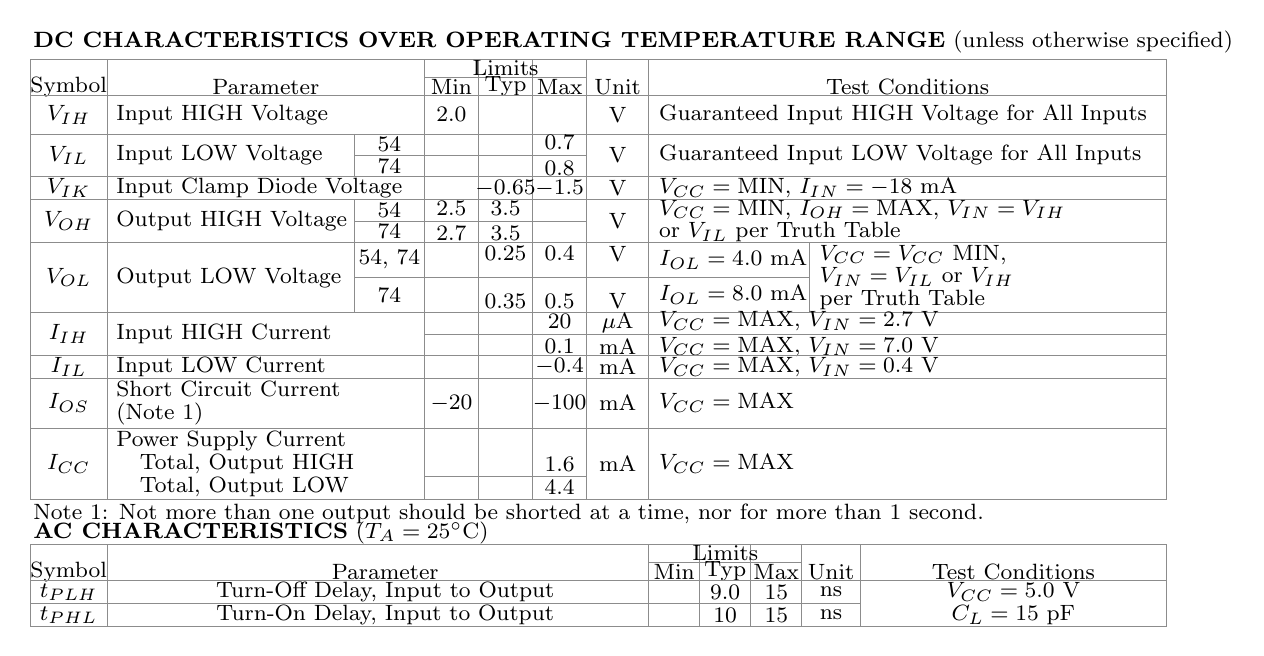
\begin{tikzpicture}[x=.982cm,y=-.97cm,font=\fontsize{8}{8.2}\selectfont]
\node[anchor=west,align=left,inner sep=1pt]at(0.0,0){\textbf{DC CHARACTERISTICS OVER OPERATING TEMPERATURE RANGE} (unless otherwise specified)};
\draw[black!45,line width=.25pt](0.0,0.23)--(0.0,6.0);
\draw[black!45,line width=.25pt](1.0,0.23)--(1.0,6.0);
\draw[black!45,line width=.25pt](5.1,0.23)--(5.1,6.0);
\draw[black!45,line width=.25pt](5.800000000000001,0.23)--(5.800000000000001,6.0);
\draw[black!45,line width=.25pt](6.5,0.23)--(6.5,6.0);
\draw[black!45,line width=.25pt](7.2,0.23)--(7.2,6.0);
\draw[black!45,line width=.25pt](8.0,0.23)--(8.0,6.0);
\draw[black!45,line width=.25pt](14.7,0.23)--(14.7,6.0);
\draw[black!45,line width=.25pt](0.0,0.23)--(14.7,0.23);
\draw[black!45,line width=.25pt](5.1,0.47)--(7.2,0.47);
\node[align=center,inner sep=1pt]at(6.15,0.35){Limits};
\node[align=center,inner sep=1pt]at(0.5,0.59){Symbol};
\node[align=center,inner sep=1pt]at(3.0499999999999994,0.59){Parameter};
\node[align=center,inner sep=1pt]at(5.45,0.59){Min};
\node[align=center,inner sep=1pt]at(6.15,0.59){Typ};
\node[align=center,inner sep=1pt]at(6.8500000000000005,0.59){Max};
\node[align=center,inner sep=1pt]at(7.6000000000000005,0.59){Unit};
\node[align=center,inner sep=1pt]at(11.350000000000001,0.59){Test Conditions};
\draw[black!45,line width=.25pt](0.0,0.71)--(14.7,0.71);
\node[align=center,inner sep=1pt]at(0.5,0.96){$V_{IH}$};
\node[anchor=west,align=left,text width=4.0cm,inner sep=1pt]at(1.0745454545454547,0.96){Input HIGH Voltage};
\node[align=center,inner sep=1pt]at(5.45,0.96){2.0};
\node[align=center,inner sep=1pt]at(6.15,0.96){};
\node[align=center,inner sep=1pt]at(6.8500000000000005,0.96){};
\node[align=center,inner sep=1pt]at(7.6000000000000005,0.96){V};
\node[anchor=west,align=left,text width=6.4cm,inner sep=1pt]at(8.0943661971831,0.96){Guaranteed Input HIGH Voltage for All Inputs};
\draw[black!45,line width=.25pt](0.0,1.21)--(14.7,1.21);
\node[align=center,inner sep=1pt]at(0.5,1.49){$V_{IL}$};
\node[anchor=west,align=left,text width=3.1cm,inner sep=1pt]at(1.0745454545454547,1.49){Input LOW Voltage};
\node[align=center,inner sep=1pt]at(5.45,1.49){};
\node[align=center,inner sep=1pt]at(6.15,1.49){};
\node[align=center,inner sep=1pt]at(6.8500000000000005,1.49){0.7\\[1pt]0.8};
\node[align=center,inner sep=1pt]at(7.6000000000000005,1.49){V};
\node[anchor=west,align=left,text width=6.4cm,inner sep=1pt]at(8.0943661971831,1.49){Guaranteed Input LOW Voltage for All Inputs};
\draw[black!45,line width=.25pt](4.194805194805195,1.21)--(4.194805194805195,1.77);
\node[align=center,inner sep=1pt]at(4.647402597402598,1.35){54};
\node[align=center,inner sep=1pt]at(4.647402597402598,1.63){74};
\draw[black!45,line width=.25pt](4.194805194805195,1.49)--(7.2,1.49);
\draw[black!45,line width=.25pt](0.0,1.77)--(14.7,1.77);
\node[align=center,inner sep=1pt]at(0.5,1.92){$V_{IK}$};
\node[anchor=west,align=left,text width=4.0cm,inner sep=1pt]at(1.0745454545454547,1.92){Input Clamp Diode Voltage};
\node[align=center,inner sep=1pt]at(5.45,1.92){};
\node[align=center,inner sep=1pt]at(6.15,1.92){$-0.65$};
\node[align=center,inner sep=1pt]at(6.8500000000000005,1.92){$-1.5$};
\node[align=center,inner sep=1pt]at(7.6000000000000005,1.92){V};
\node[anchor=west,align=left,text width=6.4cm,inner sep=1pt]at(8.0943661971831,1.92){$V_{CC}=\mathrm{MIN}$, $I_{IN}=-18$ mA};
\draw[black!45,line width=.25pt](0.0,2.07)--(14.7,2.07);
\node[align=center,inner sep=1pt]at(0.5,2.3499999999999996){$V_{OH}$};
\node[anchor=west,align=left,text width=3.1cm,inner sep=1pt]at(1.0745454545454547,2.3499999999999996){Output HIGH Voltage};
\node[align=center,inner sep=1pt]at(5.45,2.3499999999999996){2.5\\[1pt]2.7};
\node[align=center,inner sep=1pt]at(6.15,2.3499999999999996){3.5\\[1pt]3.5};
\node[align=center,inner sep=1pt]at(6.8500000000000005,2.3499999999999996){};
\node[align=center,inner sep=1pt]at(7.6000000000000005,2.3499999999999996){V};
\node[anchor=west,align=left,text width=6.4cm,inner sep=1pt]at(8.0943661971831,2.3499999999999996){$V_{CC}=\mathrm{MIN}$, $I_{OH}=\mathrm{MAX}$, $V_{IN}=V_{IH}$\\or $V_{IL}$ per Truth Table};
\draw[black!45,line width=.25pt](4.194805194805195,2.07)--(4.194805194805195,2.63);
\node[align=center,inner sep=1pt]at(4.647402597402598,2.21){54};
\node[align=center,inner sep=1pt]at(4.647402597402598,2.4899999999999998){74};
\draw[black!45,line width=.25pt](4.194805194805195,2.3499999999999996)--(7.2,2.3499999999999996);
\draw[black!45,line width=.25pt](0.0,2.63)--(14.7,2.63);
\node[align=center,inner sep=1pt]at(0.5,3.09){$V_{OL}$};
\node[anchor=west,align=left,text width=3.1cm,inner sep=1pt]at(1.0745454545454547,3.09){Output LOW Voltage};
\node[align=center,inner sep=1pt]at(5.45,3.09){};
\node[align=center,inner sep=1pt]at(6.15,3.09){0.25\\[9pt]0.35};
\node[align=center,inner sep=1pt]at(6.8500000000000005,3.09){0.4\\[9pt]0.5};
\node[align=center,inner sep=1pt]at(7.6000000000000005,3.09){V\\[9pt]V};
\node[anchor=west,align=left,text width=6.4cm,inner sep=1pt]at(8.0943661971831,3.09){};
\draw[black!45,line width=.25pt](4.194805194805195,2.63)--(4.194805194805195,3.55);
\node[align=center,inner sep=1pt]at(4.647402597402598,2.86){54, 74};
\node[align=center,inner sep=1pt]at(4.647402597402598,3.32){74};
\draw[black!45,line width=.25pt](4.194805194805195,3.09)--(7.2,3.09);
\draw[black!45,line width=.25pt](0.0,3.55)--(14.7,3.55);
\draw[black!45,line width=.25pt](7.2,3.09)--(10.07605633802817,3.09);
\draw[black!45,line width=.25pt](10.07605633802817,2.63)--(10.07605633802817,3.55);
\node[anchor=west,align=left,inner sep=1pt]at(8.0943661971831,2.86){$I_{OL}=4.0$ mA};
\node[anchor=west,align=left,inner sep=1pt]at(8.0943661971831,3.32){$I_{OL}=8.0$ mA};
\node[anchor=west,align=left,text width=4.1cm,inner sep=1pt]at(10.17042253521127,3.09){$V_{CC}=V_{CC}\ \mathrm{MIN}$,\\$V_{IN}=V_{IL}$ or $V_{IH}$\\per Truth Table};
\node[align=center,inner sep=1pt]at(0.5,3.83){$I_{IH}$};
\node[anchor=west,align=left,text width=4.0cm,inner sep=1pt]at(1.0745454545454547,3.83){Input HIGH Current};
\node[align=center,inner sep=1pt]at(5.45,3.83){};
\node[align=center,inner sep=1pt]at(6.15,3.83){};
\node[align=center,inner sep=1pt]at(6.8500000000000005,3.83){20\\[1pt]0.1};
\node[align=center,inner sep=1pt]at(7.6000000000000005,3.83){$\mu$A\\[1pt]mA};
\node[anchor=west,align=left,text width=6.4cm,inner sep=1pt]at(8.0943661971831,3.83){$V_{CC}=\mathrm{MAX}$, $V_{IN}=2.7$ V\\[1pt]$V_{CC}=\mathrm{MAX}$, $V_{IN}=7.0$ V};
\draw[black!45,line width=.25pt](0.0,4.109999999999999)--(14.7,4.109999999999999);
\draw[black!45,line width=.25pt](5.1,3.83)--(14.7,3.83);
\node[align=center,inner sep=1pt]at(0.5,4.26){$I_{IL}$};
\node[anchor=west,align=left,text width=4.0cm,inner sep=1pt]at(1.0745454545454547,4.26){Input LOW Current};
\node[align=center,inner sep=1pt]at(5.45,4.26){};
\node[align=center,inner sep=1pt]at(6.15,4.26){};
\node[align=center,inner sep=1pt]at(6.8500000000000005,4.26){$-0.4$};
\node[align=center,inner sep=1pt]at(7.6000000000000005,4.26){mA};
\node[anchor=west,align=left,text width=6.4cm,inner sep=1pt]at(8.0943661971831,4.26){$V_{CC}=\mathrm{MAX}$, $V_{IN}=0.4$ V};
\draw[black!45,line width=.25pt](0.0,4.409999999999999)--(14.7,4.409999999999999);
\node[align=center,inner sep=1pt]at(0.5,4.734999999999999){$I_{OS}$};
\node[anchor=west,align=left,text width=4.0cm,inner sep=1pt]at(1.0745454545454547,4.734999999999999){Short Circuit Current\\(Note 1)};
\node[align=center,inner sep=1pt]at(5.45,4.734999999999999){$-20$};
\node[align=center,inner sep=1pt]at(6.15,4.734999999999999){};
\node[align=center,inner sep=1pt]at(6.8500000000000005,4.734999999999999){$-100$};
\node[align=center,inner sep=1pt]at(7.6000000000000005,4.734999999999999){mA};
\node[anchor=west,align=left,text width=6.4cm,inner sep=1pt]at(8.0943661971831,4.734999999999999){$V_{CC}=\mathrm{MAX}$};
\draw[black!45,line width=.25pt](0.0,5.06)--(14.7,5.06);
\node[align=center,inner sep=1pt]at(0.5,5.529999999999999){$I_{CC}$};
\node[anchor=west,align=left,text width=4.0cm,inner sep=1pt]at(1.0745454545454547,5.529999999999999){Power Supply Current\\\quad Total, Output HIGH\\\quad Total, Output LOW};
\node[align=center,inner sep=1pt]at(5.45,5.529999999999999){};
\node[align=center,inner sep=1pt]at(6.15,5.529999999999999){};
\node[align=center,inner sep=1pt]at(6.8500000000000005,5.529999999999999){};
\node[align=center,inner sep=1pt]at(7.6000000000000005,5.529999999999999){mA};
\node[anchor=west,align=left,text width=6.4cm,inner sep=1pt]at(8.0943661971831,5.529999999999999){$V_{CC}=\mathrm{MAX}$};
\draw[black!45,line width=.25pt](0.0,6.0)--(14.7,6.0);
\node[align=center,inner sep=1pt]at(6.8500000000000005,5.529999999999999){1.6};
\node[align=center,inner sep=1pt]at(6.8500000000000005,5.84){4.4};
\draw[black!45,line width=.25pt](5.1,5.6899999999999995)--(7.2,5.6899999999999995);
\node[anchor=west,align=left,inner sep=1pt]at(0.0,6.19){Note 1: Not more than one output should be shorted at a time, nor for more than 1 second.};
\node[anchor=west,align=left,inner sep=1pt]at(0.0,6.43){\textbf{AC CHARACTERISTICS} ($T_A=25^\circ$C)};
\draw[black!45,line width=.25pt](0.0,6.58)--(0.0,7.66);
\draw[black!45,line width=.25pt](1.0,6.58)--(1.0,7.66);
\draw[black!45,line width=.25pt](8.0,6.58)--(8.0,7.66);
\draw[black!45,line width=.25pt](8.66056338028169,6.58)--(8.66056338028169,7.66);
\draw[black!45,line width=.25pt](9.32112676056338,6.58)--(9.32112676056338,7.66);
\draw[black!45,line width=.25pt](9.981690140845071,6.58)--(9.981690140845071,7.66);
\draw[black!45,line width=.25pt](10.73661971830986,6.58)--(10.73661971830986,7.66);
\draw[black!45,line width=.25pt](14.7,6.58)--(14.7,7.66);
\draw[black!45,line width=.25pt](0.0,6.58)--(14.7,6.58);
\draw[black!45,line width=.25pt](8.0,6.82)--(9.981690140845071,6.82);
\node[align=center,inner sep=1pt]at(8.990845070422536,6.7){Limits};
\node[align=center,inner sep=1pt]at(0.5,6.94){Symbol};
\node[align=center,inner sep=1pt]at(4.594155844155843,6.94){Parameter};
\node[align=center,inner sep=1pt]at(8.330281690140845,6.94){Min};
\node[align=center,inner sep=1pt]at(8.990845070422536,6.94){Typ};
\node[align=center,inner sep=1pt]at(9.651408450704226,6.94){Max};
\node[align=center,inner sep=1pt]at(10.359154929577464,6.94){Unit};
\node[align=center,inner sep=1pt]at(12.71830985915493,6.94){Test Conditions};
\draw[black!45,line width=.25pt](0.0,7.0600000000000005)--(14.7,7.0600000000000005);
\draw[black!45,line width=.25pt](0.0,7.36)--(10.73661971830986,7.36);
\draw[black!45,line width=.25pt](0.0,7.66)--(14.7,7.66);
\node[align=center,inner sep=1pt]at(0.5,7.21){$t_{PLH}$};
\node[align=center,inner sep=1pt]at(4.594155844155843,7.21){Turn-Off Delay, Input to Output};
\node[align=center,inner sep=1pt]at(8.990845070422536,7.21){9.0};
\node[align=center,inner sep=1pt]at(9.651408450704226,7.21){15};
\node[align=center,inner sep=1pt]at(10.359154929577464,7.21){ns};
\node[align=center,inner sep=1pt]at(0.5,7.51){$t_{PHL}$};
\node[align=center,inner sep=1pt]at(4.594155844155843,7.51){Turn-On Delay, Input to Output};
\node[align=center,inner sep=1pt]at(8.990845070422536,7.51){10};
\node[align=center,inner sep=1pt]at(9.651408450704226,7.51){15};
\node[align=center,inner sep=1pt]at(10.359154929577464,7.51){ns};
\node[align=center,inner sep=1pt]at(12.71830985915493,7.36){$V_{CC}=5.0$ V\\$C_L=15$ pF};
\end{tikzpicture}
